% \vspace{-5pt}
\section{Reasoning via Planning (RAP)}
% \vspace{-5pt}

% Most recent LLMs use an autoregressive decoder architecture when solving reasoning tasks, which prevents them from looking ahead and doing exploration when making a reasoning step.
% This inability may be blamed for their failures on complex multi-step reasoning tasks.
% To address these shortages, we propose to form reasoning as a planning task. In this section, we will introduce the world model formulation (how to look ahead?), and the search algorithm (how to do exploration?). \gy{modify this paragraph ; we do not want to use look ahead}


% During the process of solving complex reasoning problems, humans frequently engage in planning by simulating each step of the reasoning process using the world model in their minds.
% They iterate through recognizing problematic steps and exploring alternative reasoning steps to enhance the overall reasoning path.
% % \gy{unsure whether the description is accurate}
% However, existing approaches that employ LLMs to tackle reasoning problems solely rely on autoregressive generation of the reasoning trace, preventing them from recovering from incorrect early steps and exploring alternative paths.

% In order to overcome the limitations arising from this discrepancy,

% \subsection{Planning with Monte Carlo Tree Search} \label{sec:mcts}







In this section, we present the Reasoning via Planning (RAP) framework that enables LLMs to strategically plan a coherent reasoning trace for solving a wide range of reasoning tasks. We first \roundinlinebox[green]{build the world model} by repurposing the LLM with prompting (Section~\ref{sec:formulation}). The world model serves as the foundation for deliberate planning, by allowing the LLM to plan ahead and seek out the expected outcomes in the future. We then introduce the \roundinlinebox[green]{rewards} for assessing each state during reasoning in Section~\ref{sec:reward}. Guided by the world model and rewards, the planning with \roundinlinebox[green]{Monte Carlo Tree Search} (MCTS) efficiently explores the vast reasoning space and finds optimal reasoning traces (Section~\ref{sec:mcts}). Finally, when multiple promising reasoning traces are acquired during planning, we further introduce an aggregation method in Section~\ref{sec:aggr} that yields an ensembled result and further boosts the reasoning performance.

% which simulates each step of the reasoning trace, as described in Section \ref{sec:formulation}.
% This world model not only provides the outcome of the reasoning step but also evaluates its effectiveness, as described in Section \ref{sec:formulation}.
% We then discuss how to evaluate the effectiveness of reasoning steps to provide rewards in Section \ref{sec:reward}.
% Subsequently, we present our planning algorithm adapted from the Monte Carlo Tree Search (MCTS) algorithm to perform {planning} of the reasoning trace using the world model, as outlined in Section \ref{sec:mcts}.
% Finally, when multiple promising reasoning traces are explored during the planning process, we further introduce RAP-aggregate in Section \ref{sec:aggr} to select the best answer by aggregating these reasoning traces.

% drawing inspiration from the human ability to validate results by considering multiple reasoning traces~\cite{wang2022self}, we introduce RAP-aggregate in Section \ref{sec:aggr}. RAP-aggregate enables the selection of the best answer by aggregating the results obtained from multiple reasoning traces explored during the planning process.



% In this paper, we propose a new framework of LLM reasoning, namely \textbf{Reasoning via Planning (RAP)}, which leverage the LLM as both a world model and an agent.
% In Section \ref{sec:formulation}, we describe how to employ a LLM as the world model to explicitly predicts the next state and reward at each reasoning steps, transforming a reasoning task into a problem of planning.
% In Section \ref{sec:mcts}, we demonstrate how an agent LLM model, with the powerful feedback from the world model, can strategically plan a reasoning trace using the Monte Carlo Tree Search algorithm \cite{browne2012survey}.
% We finally introduce RAP-aggregate in Section \ref{sec:aggr}, which can aggregate a best answer across multiple reasoning traces we find during the planning.

%\vspace{-5pt}
\subsection{Language Model as World Model}
\label{sec:formulation}
%\vspace{-5pt}


%https://courses.cs.washington.edu/courses/cse599i/18wi/resources/lecture19/lecture19.pdf

% \begin{figure}[t]
%     \centering
%     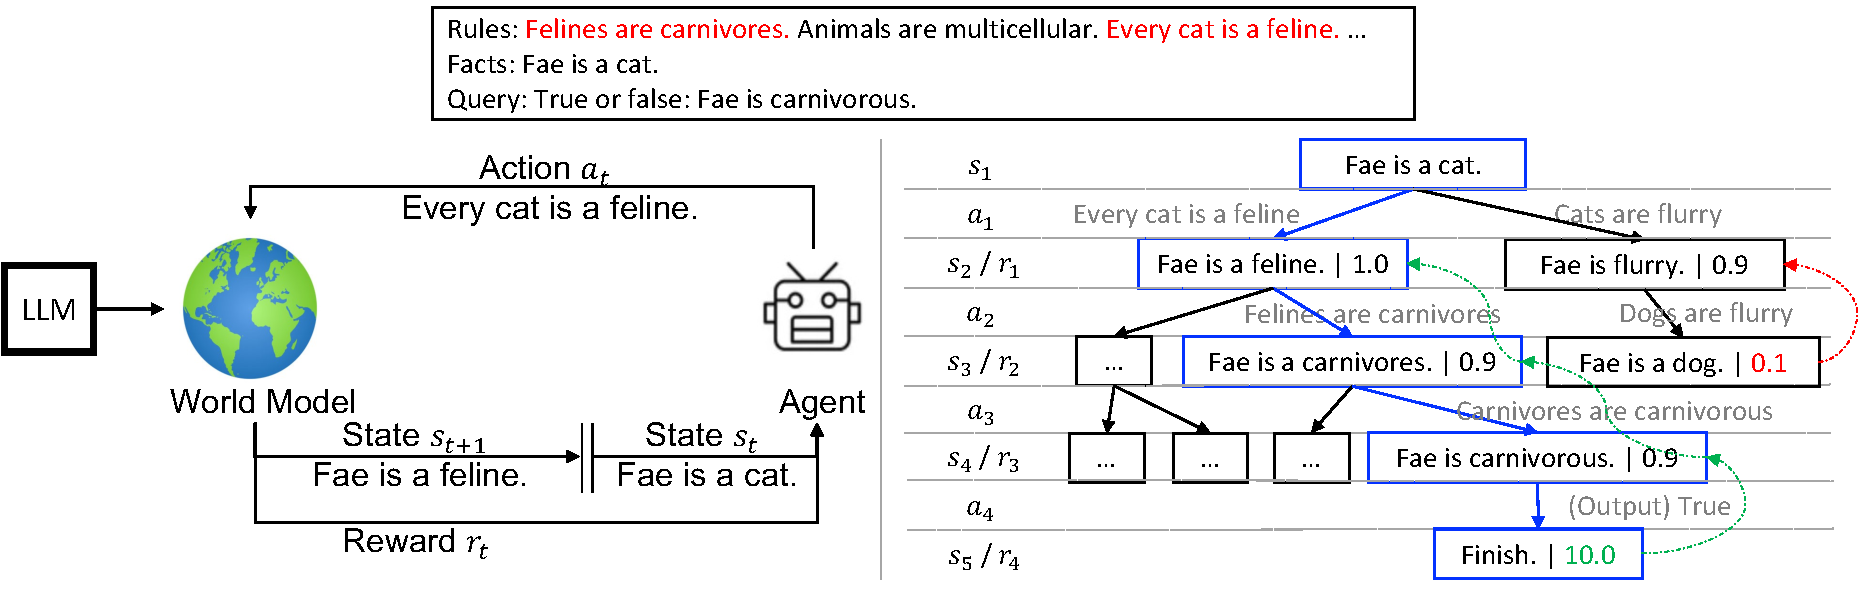
\includegraphics[width=\textwidth]{sections/fig_formulation.pdf}
%     \caption{Formulation of RAP in an example from PrOntoQA. The left is the formulation of LLM as World Model, and the right is a search tree in this example.}
%     \label{fig:formulation}
% \end{figure}

In general, a world model predicts the next \emph{state} of the reasoning after \roundinlinebox[green]{applying an \emph{action} to the current state}~\cite{ha2018world, matsuo2022deep}. \ours enables us to instantiate the general concepts of state and action in different ways depending on the specific reasoning problems at hand (Figure \ref{fig:tree_examples}). For example, in \blocksworld, it is natural to define a state as the configuration of blocks (described in natural language), and an action to be a behavior of moving a block (e.g., ``pickup the orange block''). In a math reasoning problem, we use the state to represent the values of intermediate variables, and set an action to be a subquestion that drives the reasoning to derive new values. In logical reasoning, a state is a fact we are focusing on, and an action is to choose a rule for the next deduction.


With the definition of state and action, the reasoning process can thus be described as a \roundinlinebox[green]{Markov decision process (MDP):} given the current state $s_{t, t=0, 1, \dots, T}$, e.g., the initial state $s_0$, the LLM (as a reasoning agent) generates an action space by sampling from its generative distribution $a_t \sim p(a | s_t, c)$, where $c$ is a proper prompt (e.g., in-context demonstrations). Once an action is chosen, the world model then predicts the next state $s_{t+1}$ of the reasoning. Specifically, we repurpose the \emph{same} LLM to obtain a state transition distribution $p(s_{t+1} | s_t, a_t, c')$, where $c'$ is another prompt to guide the LLM to generate a state. For instance, in \blocksworld, the LLM (as the world model) generates text $s_{t+1}$ to describe the new configuration of blocks, given previous state $s_{t}$ and the action $a_t$.

Continuing the process results in a reasoning trace, which consists of a sequence of interleaved states and actions $(s_0, a_0, s_1, \dots, a_{T-1}, s_T)$. This differs from the previous reasoning methods, such as Chain-of-Thought~\cite{wei2022chain}, where the intermediate reasoning steps consist of only a sequence of actions, e.g., (\texttt{$a_0=$ ``pickup red block'', $a_1=$ ``stack on yellow block'',} \dots) (see comparisons in Figure~\ref{fig:1}). Augmenting the reasoning with the (predicted) world states helps the LLM with a more grounded and coherent inference. Note that the full reasoning trace is simulated by the LLM itself (as a reasoning agent with an \emph{internal} world model) without interacting with the \emph{external} real environment. \highlight[green]{This resembles humans contemplating a possible plan in their minds. The capability of simulating future states, by introducing the world model, allows us to incorporate principled planning algorithms to efficiently explore the vast reasoning space} as described in Section~\ref{sec:mcts}.


% To introduce the world model for simulating reasoning traces, we begin by defining the concepts of \textit{states} and \textit{actions} within a reasoning task.
% % We illustrate this with an example taken from the PrOntoQA dataset \cite{saparov2022language}, as shown in Figure \ref{fig:formulation}.
% We illustrate this with an example derived from the \blocksworld benchmark \cite{valmeekam2022large}.
% In our approach, we represent the reasoning process as a Markov decision process (MDP) with a state space $\mathcal S$ and an action space $\mathcal A$, as depicted in Figure \gy{ref figure}. %\ref{fig:formulation} (left).
% Each state $s \in \mathcal S$ corresponds to an intermediate status in the reasoning, specifically a language description of the current configurations of blocks in the \blocksworld context. %``\texttt{Fae is a cat}''.
% % At time $t$, an agent proposes an action $a_t \in \mathcal A$, which represents a rule to be employed in the subsequent reasoning step, such as ``\texttt{Every cat is a feline}'', based on the current state $s_t$ and its policy $p_\phi(a \mid s_t)$.
% At time $t$, an agent proposes an action $a_t \in \mathcal A$, which represents the subsequent reasoning step, such as a movement of a single block, based on the current state $s_t$ and its policy $p(a \mid s_t)$.
% The world model then conducts a one-hop reasoning step using $s_t$ and $a_t$, transitioning the state into the subsequent state $s_{t+1}$, which in this case denotes the new configuration of blocks after performing the movement $a_t$ on the current configuration $s_t$.
% The specific definition of states and actions can vary depending on the nature of the reasoning task.
% For example, in GSM8k \cite{cobbe2021training}, a dataset of numerical reasoning, the action is defined as proposing an incremental sub-question, while the state comprises the history of previous sub-questions and their corresponding answers.
% In terms of state transition, the world model attempts to answer the sub-question based on the problem context and the current state, subsequently incorporating the answer into the history to form the next state.

% In order to enable the world model to predict state transitions, which are subsequently utilized by agents for planning, we leverage the LLM as the state transition probability function $p_\theta$.
% In the \blocksworld example, we prompt the LLM the domain rule, the state $s_t$, the action $a_t$, and few-shot examples, to predict the next state $s_{t+1}$.




% In the PrOntoQA example, we prompt the LLM the state $s_t$ and action $a_t$ with few-shot examples to get the next state $s_{t+1}$.
% We also prompt it ``\texttt{Is this reasoning step correct?}'', and use the probability of ``\texttt{Yes}'' as the reward, evaluating the correctness of this reasoning step.

%However, the LLM often makes mistakes in retrieving accurate information or performing correct mathematical calculations.
%To ensure the reliability of our world model, we sample the LLM multiple times and select the next state with the highest confidence (The frequency of an answer). \gy{OK to directly say confidence?}
%We also use this confidence value as a reward, discouraging excessively difficulty or skipping sub-questions.

% In plan generation tasks, the world model is used to simulate actions by predicting the state transitions and the rewards without requiring direct access to the environment.
% In numerical and logical reasoning tasks, the LLM is utilized to answer sub-questions and perform atomic logical reasoning steps, allowing us to learn the outcome of reasoning steps and providing evaluations how good they are.
% Through the integration of the world model, a reasoning task is transformed into a strategic planning problem over the MDP, guided by the rewards.

% To address this, we employ a LLM as the world model, leveraging it to simulate the state transition function and the reward function.
% In abstract reasoning tasks \gy{unsure how to describe this type}, the definition of states and actions are more flexible.
% A partial solution $s \in \mathcal S$ can correspond to an intermediate conclusion or the previous answers of decomposed sub-questions. A reasoning step $a \in \mathcal A$ can refer to a given fact or a new sub-question that leads to the next state.
% In these cases, we also utilize a LLM as the world model to simulate the state transition, enabling us to derive the next intermediate conclusion or answer the sub-question. We also evaluate the quality of each reasoning step using the LLM as the reward function.
% We illustrate the detailed MDP formulations of Blocksworld, ProntoQA, and GSM8k in \gy{table/figure}. \gy{we want to include action proposing in world model, need modify}

% We assume the MDP has finite horizon, which means any transition sequence of nonzero probability (i.e. $ \prod_{i \geq 0} \mathcal{P}\left(x_i, a_{i, i+1}, x_{i+1}\right)>0$) must have finite length.
% Since their concrete interpretations of the MDP depend on specific problems, we leave them to later sections \hsb{ref}. Here we take a case from blockworld as a running example: \hsb{expand}

% In our method, the transition probability function and the reward function are parameterized by the world model, noted as $\mathcal{P_\phi}$ and $\mathcal{R_\phi}$. \hsb{example}

% A planning problem is formulated as below:


%\vspace{-5pt}
\subsection{Reward Design} \label{sec:reward}
%\vspace{-5pt}

During reasoning, we want to assess the feasibility and desirability of each reasoning step, and guide the reasoning based on the assessment (Section~\ref{sec:mcts}).
The assessment of each reasoning step (i.e., applying an action $a_t$ to the state $s_{t}$) is performed by a \emph{reward} function $r_t = r(s_t, a_t) \in \mathbb R$. Similar to the state and action, the reward function can be specified in different ways to accommodate any knowledge or preferences about the reasoning problem of interest. Here we introduce several common rewards applicable to different tasks and shown to be effective in our experiments.

\noindent \textbf{Likelihood of the action.}
When an action is generated by the LLM conditioning on the in-context demonstration and the current state, the probability of the specific action reflects the LLM's preference. We thus can incorporate the log probability of the action as a reward. This reward reflects the ``instinct'' of LLMs as an agent, and can be also used as a prior for which action to explore.

\noindent \textbf{Confidence of the state.}
State prediction is nontrivial in some problems, e.g., in math reasoning (Figure~\ref{fig:tree_examples}, middle), given an action (i.e., a subquestion), the world model predicts the next state by answering the subquestion. We incorporate the confidence of the state (i.e., answers in this case) as a reward. Specifically, we draw multiple sample answers from the world model, and use the proportion of the most frequent answer as the confidence. Higher confidence indicates that the state prediction is more consistent with the world knowledge of LLMs \cite{hao2023bertnet}, which typically leads to a more reliable reasoning step.

% In certain tasks, individual reasoning step can still be challenging.
% For example, in the GSM8k dataset \cite{cobbe2021training}, a reasoning step involves proposing (action) and answering a sub-question (state transition) based on previous information.
% We then use the confidence of answers as a reward. Specifically, we sample multiple responses from the world model and group them by the answer. The maximal frequency of an answer is defined as confidence, and high confidence indicates reliable reasoning steps.

% \textbf{Correctness estimation by LLM. \gy{Since we use this way to calculate correctness in PrOntoQA and helpfulness in GSM8k, shall we replace with `Self-evaluation by LLM'} \hzt{sounds good. and please update the paragraph}}
\noindent \textbf{Self-evaluation by the LLM.}
It's sometimes easier to recognize the errors in reasoning than avoid generating them in advance. Thus, it's beneficial to allow the LLM to criticize itself with the question ``\texttt{Is this reasoning step correct?}'', and use the next-word probability of the token ``\texttt{Yes}'' as a reward. The reward evaluates LLM's own estimation of the correctness of reasoning. Note that the specific problems for self-evaluation can be different depending on the tasks.

% Likewise, we can prompt the LLM with the question ``\texttt{Is this reasoning step correct?}'' and utilize the probability of the token \texttt{Yes} as a reward, reflecting the LLM's evaluation of the reasoning step's reliability,

\noindent \textbf{Task-specific heuristics.}
RAP also allows us to flexibly plug in other task-specific heuristics into the reward function. For example, in plan generation for \blocksworld, we compare the predicted current state of blocks with the goal to calculate a reward (Section~\ref{sec:plan}). The reward encourages the plan of movements to actively pace towards the target.

% In plan generation tasks, we can also borrow the rewards from the corresponding environment. For example, in \blocksworld benchmark \cite{valmeekam2022large}, we can assign reward by the number of sub-goals that are fulfilled when performing the movement in action $a_t$.

% As a by-product, the new state is predicted as the ensemble of multiple samples, which may better align with the LLM's belief about the world \cite{jung2022maieutic, hao2022bertnet}.



% Besides the world model, we define a reward function $r_t = r(s_t, a_t) \in \mathbb R$ for each task to assess the quality of this reasoning step.
% The reward function can incorporate various evaluation approaches, some of which are outlined below.

% \vspace{-5pt}
\subsection{Planning with Monte Carlo Tree Search} \label{sec:mcts}
% \vspace{-5pt}


\begin{figure*}[t]
    \centering
    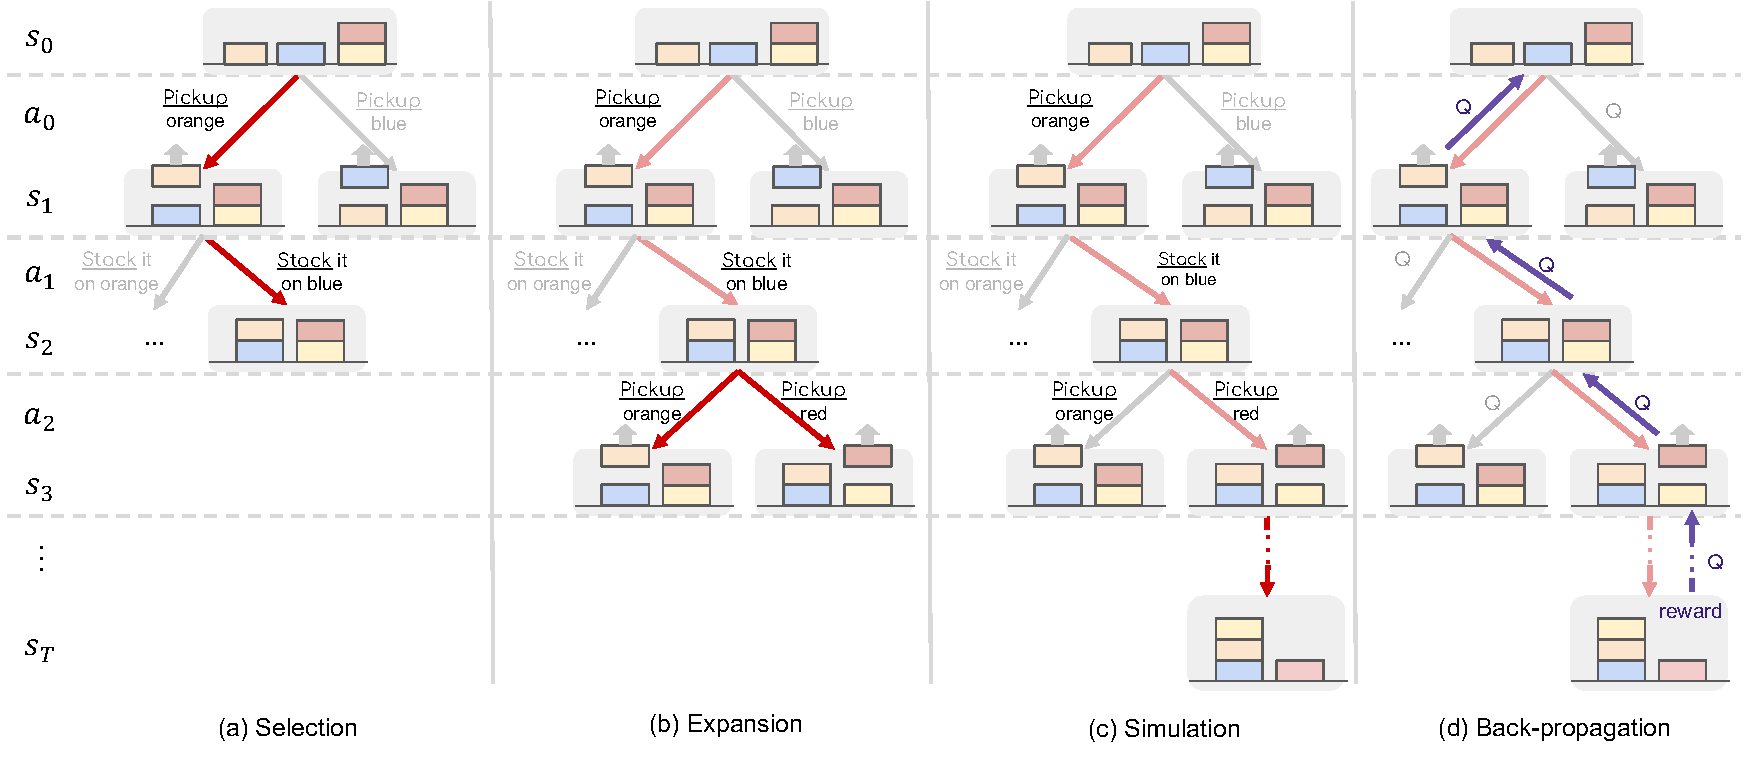
\includegraphics[width=\textwidth]{sections/mcts_phases.pdf}
    \vspace{-25pt}
    \caption{An illustration of the four phases in an iteration in MCTS planning (Section~\ref{sec:mcts}).}
    \label{fig:mcts_phases}
    \vspace{-12pt}
\end{figure*}


Once equipped with the world model (Section~\ref{sec:formulation}) and rewards (Section~\ref{sec:reward}), LLMs can reason with any planning algorithms. We adopt Monte Carlo Tree Search (MCTS)~\cite{kocsis2006bandit, coulom2007efficient}, a powerful planning algorithm that strategically explores the space of reasoning trees and strikes a proper balance between exploration and exploitation to find high-reward reasoning traces efficiently.

Specifically, MCTS builds a reasoning tree iteratively, where each node represents a state, and each edge represents an action and the transition from the current state to the next state after applying the action (Figure~\ref{fig:1}).
To guide the LLM agent to expand and explore the most promising nodes of the tree, the algorithm maintains a state-action value function $Q : \mathcal S \times \mathcal A \mapsto \mathbb R$, where $Q(s, a)$ estimates the \emph{expected future reward} of taking action $a$ in state $s$. Figure \ref{fig:mcts_phases} illustrates four operations in each iteration to expand the tree and update $Q$ values. The process continues until a specified computational budget (e.g., the number of iterations) is reached, and the resulting traces are acquired from the tree. More details and the pseudo-code of the planning algorithm are given in Appendix~\ref{sec:mcts_app} and Algorithm \ref{alg:mcts}.


% That is, we assess the potential of a node (a reasoning step) by looking ahead and anticipating the reward in future trajectories starting from this node. This fundamentally differs from the current reasoning methods that generate a reasoning trace autoregressively without considering the future.


% More specifically, as illustrated in Figure \ref{fig:mcts_phases}, the MCTS planning performs four operations in each iteration to expand the tree and update $Q$ values, i.e., \textit{selection}, \textit{expansion}, \textit{simulation}, and \textit{back-propagation}. The process continues until a specified computational budget (e.g., the number of iterations) is reached, and the resulting reasoning traces are acquired from the tree, as we articulated later. The psuedo-code of our MCTS planning is given in Algorithm \ref{alg:mcts} in the Appendix.
% The iterations continue until a target state is reached, resulting in a complete reasoning trace for the target problem.

% We employ Monte Carlo Tree Search (MCTS), a decision-making algorithm that explores the MDPs using a decision tree, by which we can balance exploration and exploitation when planning the reasoning trace. In the decision tree representation, each node represents a state, while each edge represents an action and the corresponding state transition, as illustrated in Figure \ref{fig:formulation} (right).

% The algorithm maintains an optimal state-action value function $Q : \mathcal S \times \mathcal A \mapsto \mathbb R$, where $Q(s, a)$ estimates the maximum expected reward starting from state $s$ with action $a$.
% MCTS operates iteratively by sampling a complete trajectory (i.e., a reasoning trace) from the root of the tree (initial state $s_0$) towards a terminating node, where the agent finishes the reasoning.
% This iterative process expands the decision tree incrementally with each iteration.
% Additionally, the $Q$ values of the state-action pairs along the trajectory are updated in each iteration.
% Every iteration is composed four phases, \textit{selection}, \textit{expansion}, \textit{simulation}, and \textit{back-propagation}, demonstrated in Algorithm \ref{alg:mcts} with details below.

% In reasoning tasks, the state space and action space of half-way solutions can be very large and even infinite due to the flexibility to propose reasoning steps in natural language, which means that the state space cannot be fully searched.
% In order to do planning on the MDP within a computational budget, we introduce the Monte Carlo Tree Search algorithm \cite{browne2012survey} to strategically and efficiently search for a good plan.
% The algorithm builds a rooted tree of the search history, where each node represents a state, while each edge represents an action.
% It also maintains an optimal state-action value function $Q: \mathcal S \times \mathcal A \mapsto \mathbb R$, which will be used in roll-out policy.
% The algorithm will do several iterations, called roll-outs, each of which consists of the following four phases.
% We present the roll-out procedure in Algorithm \ref{alg:mcts} with psuedo-code.

\noindent \textbf{Selection.}
The first phase selects a portion of the existing tree that is most promising for further expansion in the next phase. Starting from the root node (i.e., initial state $s_0$), at each level of the tree, the algorithm selects a child node as the next node. The phase finishes when a leaf node of the current tree is reached. Figure~\ref{fig:mcts_phases}(a) highlights the selected path in red. To balance between exploration (of less-visited nodes) and exploitation (of high-value nodes), we use the well-known \emph{Upper Confidence bounds applied to Trees (UCT)} \cite{kocsis2006bandit} to select each child node. Specifically, at node $s$, we select the action in the tree by considering both the $Q$ value (for exploitation) and uncertainty (for exploration):

\vspace{-8pt}
{
\small
\begin{align}
    a^\ast = \arg\max_{a \in A(s)} \left[ Q(s, a) + w \sqrt{\frac{\ln N(s)}{N(c(s, a))}} \right],
\end{align}
}
\noindent where $N(s)$ is the number of times node $s$ has been visited in previous iterations, and $c(s, a)$ is the child node of applying $a$ in state $s$. The less a child node was visited before (i.e., the more uncertain about this child node), the higher the second term in the equation. The weight $w$ controls the balance between exploration and exploitation.
% \hzt{Anything to say about how we chose $w$?}

% Each iteration starts the initial state.
% In each step, the algorithm will select a child node based on a \textit{tree policy}, until reaching an unvisited node.
% To balance between exploration and exploitation, we use the maximum Upper Confidence Trees (UCT) policy, which select the child node based on maximizing upper confidence.
% The upper confidence is determined by the summation of the $Q$ value, which encourages exploitation, and an uncertainty term, which encourages exploration.
% \begin{align}
%     a^\ast = \arg\max_{a \in A(s)} \left[ Q(s, a) + w \sqrt{\frac{\ln N(s)}{N(c(s, a))}} \right],
% \end{align}
% where $N(s)$ is the number of times node $s$ has been visited, and $c(s, a)$ is the children of following $a$ at node $s$.
% The hyper-parameter $w$ serves as a balancing factor between exploration and exploitation.

\noindent \textbf{Expansion.}
This phase expands the tree by adding new child nodes to the leaf node selected above. Given the state of the leaf node, we use the LLM (as agent) to sample $d$ possible actions (e.g., subquestions in math reasoning), and then use the LLM (as world model) to predict the respective next state, resulting in $d$ child nodes. Note that if the leaf node selected above is a terminal node (the end of a reasoning chain) already, we will skip expansion and jump to back-propagation.
% Note that if the leaf node selected above is a terminal (target) state already, we will skip expansion/simulation and jump to back-propagation.

% When reaching a node that have never been visited, we add to the tree the children of the node.
% Since the space of language representations can be very large, we sample $d$ possible actions using the LLM as a substitute action space $A(s)$, and add the $d$ corresponding children to the tree.

% Since the space of action, which is a language representation of the next reasoning step, can be very large, we sample $d$ possible actions using the world model LLM as the children, where $d$ is a pre-defined hyper-parameter.
% To simplify the problem, we sample a next state using the transition probability function, and reuse the sample in the future.
% The difficulty of predicting state transitions vary among tasks.
% For easier transitions, we to generate the next state with greedy decoding, while for harder transitions, we utilize self-consistency, which means we use the next state with highest confidence across several generations.
% We will also have a quick evaluation of each action, namely a prior $r'$, which can be but not necessarily be the reward defined in the world model.
% We use $r'$ to temporarily serve as $Q(s, a)$ before a roll-out actually follows $a$ at the node representing the state $s$.

\noindent \textbf{Simulation.}
To estimate the expected future rewards ($Q$ values), this phase simulates the future situations of the current node using the world model.
% Specifically,
%from the above $d$ new nodes, we pick the node of largest local reward (Section~\ref{sec:reward}) and perform simulation starting from it. In particular, similar to above,
Starting from the current node as above, at each node $s$, we create an action following a \emph{roll-out policy} and use the world model to predict the next state. The roll-out process continues until a terminal state is reached. There could be many ways to define the roll-out policy (e.g., by adding different randomness). In our experiments, for simplicity and reduced noises, we follow a similar process as in the expansion above, i.e., generating $d$ candidate actions and picking one of the largest local reward $a'= \max_{a'} r(s, a)$. In practice, for efficiency, we discard the computationally costly components in $r$ (e.g., the reward from the confidence of state requires sampling the answer multiple times), and use the resulting lightweight reward function for selecting actions during simulation.

% In traditional MCTS algorithms, after expanding the children of one node, it will follow a random simulation till a terminating state, i.e., a leaf node.
% To encourage efficient exploration, we instead follow the children with the highest prior $r'$, and repeat this procedure after expanding the new visited node till the end.


% After expansion, we perform a complete simulation starting from the current node until the reasoning trace is finished following a \textit{roll-out policy}. To guide our exploration towards better reasoning traces, we use a fast reward function $r'(s, a)$, discarding time-consuming parts of the standard reward function $r(s, a)$, to get an estimation of the quality of action $a$. Our roll-out policy selects the action with maximum estimated reward $a_t = \max_{a_t} r'(s, a_t)$.

\noindent \textbf{Back-propagation.}
Once we reach a terminal state in the above phases, we obtain a reasoning path from the root node to the terminal node. We now back-propagate the rewards on the path to update the $Q$ value of each state-action pair along the path. Specifically, we update $Q(s, a)$ by aggregating the rewards in all future steps of node $s$.
% We may adopt the aggregation method depending on the nature of tasks and reward design, as discussed in Section~\ref{sec:experiments}.
% After an iteration reaches a terminal state in the above phases.
% We back propagated the rewards on the path, updating the $Q$ function with each state-action pair in the trajectory with rewards in all future steps.
% Since the $Q$ function depends on the reward design, we will introduce in detail in Section \ref{sec:experiments}.

Once a predetermined number of MCTS iterations is reached, we terminate the algorithm and select the final reasoning trace from the constructed tree for evaluation. There are various ways for the selection.
% Following a predetermined number of iterations, there are several strategies for selecting the final reasoning path.
One is to start from the root node and iteratively choose the action with the highest $Q$ value until reaching a terminal.
Also, one can directly select the path from the iterations that yielded the highest reward, or opt to choose the leaf node (and the respective root-to-leaf path) that has been visited the most.
In practice, we observed that the second strategy often yields the best results.

% When solving a reasoning problem in the task, we deploy an agent to search over the corresponding MDP.
% In order to keep a track of the searching history, we build a reasoning tree representing the progress of searching.
% Each node on the tree represents a state $S \in \mathcal S$ in the MDP, where the root represents the initial state $S_0$.
% Every time the agent reaches a new node $S_t$ on the tree,

%\vspace{-5pt}
\subsection{RAP-Aggregation} \label{sec:aggr}
%\vspace{-5pt}

% : Aggregating Multiple Reasoning Outputs

For problems, such as math reasoning (Section~\ref{sec:math}) where only the final answer is required, \ours could produce multiple traces and answers from different MCTS iterations, which will be aggregated to produce the final answer. We refer to such a mechanism as \ours-Aggregation. Note that problems like plan generation or logical inference require a complete reasoning trace as output; thus, \ours-Aggregation will not be applied.

% More importantly, there is a concern that some incorrect reasoning steps may appear in the early stage of multiple iterations, thus polluting the aggregation. As a result, we further devise a new weighting strategy for aggregating candidate answers. Specifically, for each candidate answer, we accumulate the reward of each reasoning step in the answer's reasoning traces. We choose the answer with the highest accumulative reward as the final aggregated answer.


% Some of the reasoning problems, such as plan generation (Section~\ref{sec:plan}) and logical inference (Section~\ref{sec:logical}), require a complete reasoning trace as output. In other problems, such as math reasoning (Section~\ref{sec:math}), only the final answer is required. In such cases, we could collect multiple reasoning traces during RAP and aggregate the respective answers to produce the final answer, similar to the self-consistency method \cite{wang2022self} in Chain-of-Thought.
% Specifically, we collect reasoning traces and answers from different MCTS iterations. To address the concern that some incorrect early reasoning steps may appear in multiple iterations and thus pollute the aggregation, we devise a new  weighting strategy for aggregating candidate answers. Specifically, for each candidate answer, we accumulate the reward of each reasoning step in the answer's reasoning traces. We choose the answer with the highest accumulative reward as the final aggregated answer.

% However, in certain tasks such as many numerical reasoning tasks, only the final answer needs to be provided.
% When tackling numerical reasoning problems, humans often consider multiple reasoning paths to verify the answer further.
% Inspired by this, we introduce \textbf{RAP-aggregation}, where we aggregate the answer across iterations to enhance the output of MCTS.
% To address the concern that an early incorrect reasoning step may contribute multiple times to the final result when it appears in multiple iterations, we perform the aggregation in a basis of edges.
% Specifically, for a given potential answer, we accumulate the weights of all edges involved in at least one iteration leading to that particular answer.
% The weight of an edge is the reward assigned to its represented action.
% Ultimately, the answer with the highest total weight is selected as the aggregated output.
% To avoid an early incorrect reasoning step contributing multiple times to the result when multiple iterations include that step, we conduct the vote by edges.
% More specifically, for one possible answer, all edges involving in at least one iteration with that final answer will be added to the weight for the answer, and the weight is the reward of the action represented by the edge.


% Formally, we choose the answer $o$ following
% \begin{align}
%     o^\ast = \arg\max_{o} \sum_{e = (s, a): \exists T: T\text{~outputs~}o \wedge e \in T} r(s, a),
% \end{align}
% where $e$ is an edge on the tree representing following action $a$ when visiting the node representing $s$, and $T$ is the trace in one roll-out.
